\documentclass[10pt]{ctexart}
\CTEXsetup[format={\Large\bfseries}]{section}
\usepackage{cite}
\usepackage{graphicx}
\usepackage{subfigure}
\usepackage{booktabs}
\usepackage{geometry}
\usepackage{float}
\usepackage{amsmath}
\usepackage{lmodern}
\usepackage{multirow}
\usepackage{CJK}
\usepackage[marginal]{footmisc}
\renewcommand{\thefootnote}{}
\usepackage{multicol} % 用于实现在同一页中实现不同的分栏
\geometry{a4paper,scale=0.8}
% \usepackage{cjk}
% \newcommand{\upcite}[1]{\textsuperscript{\textsuperscript{\cite{#1}}}}
\usepackage{authblk}
 

\newcommand{\upcite}[1]{\textsuperscript{\textsuperscript{\cite{#1}}}}
\begin{document}
\setlength{\columnsep}{25pt} 
% \author{王树立}
\date{}
\bibliographystyle{unsrt}
\title{勺型网络:用于landsat遥感图像云检测的新型网络}
\author[]{王树立\thanks{\noindent \textbf{通讯作者}: E-mail:wangshuli18@mails.ucas.ac.cn}\ , 唐海蓉}
\affil[]{\small(中国科学院空天信息创新研究院,北京 100094; 中国科学院大学,北京 100049;\\ 中国科学院空间信息处理与应用系统技术重点实验室,北京 100190)}
\renewcommand\Authands{\, }
\pagestyle{empty} % 没有页眉和页脚
\maketitle
\pagestyle{empty} % 去掉第二页及其后各页的页码
\thispagestyle{empty} % 去掉当前页的页码
% \section*{}
\noindent\textbf{摘\ 要}\ 可靠的云检测是应用遥感图像时重要的预处理步骤,一直是遥感领域中的研究热点。本文针对目前神经网络模型存在的细节信息易损失、参数量大、计算复杂等不足,提出了一种新型的、轻量的网络,称为勺型网络(Spoon-Net)。S-Net分两个阶段分别提取光谱与空间信息,第一阶段,使用1*1的卷积核对遥感图像进行光谱特征提取;第二阶段,使用3*3的卷积核对遥感图像进行空间特征提取。而且,为了更加有效地提取空间特征,避免重复计算光谱特征,本文引入分组卷积,对第一阶段提取的每一层光谱通道单独进行卷积。模型在landsat 8 biome数据做训练并估计,在模型参数量只有unet的八十分之一(0.34M)的情况下,取得了全面优于unet的实验结果,总准确率为95.34\%,UNet为94.15\%;f1值为0.9505,UNet只有0.9352。

\noindent\textbf{关键词}\ landsat, 云检测,神经网络

\noindent\textbf{中图分类号}:TP751.2

\begin{center}
    \Large
    Spoon network: A new network structure of landsat imagery cloud detection
    \\[10pt]
    \normalsize 
    Wang Shuli, Tang Hairong 
    \\[8pt]
    \small
    (Aerospace Information Research Institutue, Chinese Academy of Sciences, Beijing 100094, China;
    
    University of Chinese Academy of Sciences, Beijing 100049, China; Key Laboratory of Technology in Geo-spatial Information Processing and Application System, Beijing 100190, China)
\end{center}

\noindent\textbf{Abstract}\ Reliable cloud detection is an important preprocessing step in the application of remote sensing images, and has been a research hotspot in the field of remote sensing. In this paper, a new and lightweight neural network, called spoon net, is proposed to solve the problems of large parameters, complex calculation and easy loss of details in the current neural network model. S-Net is divided into two stages to extract spectral and spatial information. In the first stage, 1 * 1 convolution check is used to extract spectral features of remote sensing images; in the second stage, 3 * 3 convolution check is used to extract spatial features of remote sensing images. In addition, in order to extract spatial features more effectively and avoid the repeated calculation of spectral features, this paper introduces group convolution to separate each layer of spectral channels extracted in the first stage. The model is trained and estimated with Landsat 8 biome data. When the model parameters are only one eightieth (0.35m) of UNET, the experimental results are better than UNET in all respects. The total accuracy is 95.34 \%, UNET is 94.15 \%; F1 is 0.9505, UNET is only 0.9352.

\noindent\textbf{Keywords}\ landsat, cloud detection, neural network

% \columnseprule=1pt         % 实现插入分隔线
\begin{multicols}{2} 

\setcounter{section}{-1} % 从0开始计数
\section[]{引言}
卫星遥感数据在当今社会的生产和生活中扮演着至关重要的角色,在农业产量估算\upcite{prasad2006crop}、变化检测\upcite{verbesselt2010detecting}、灾难评估\upcite{joyce2009review}等方面发挥着重要的作用。随着科技的发展,遥感数据变得越来越多,且越来越容易获得。海量的多波段遥感数据也急切需要高效率和高鲁棒性的算法进行处理和数据挖掘。然而,在landsat数据集上,每年有高达40\%的像素被云覆盖\upcite{ju2008availability},云层作为光学遥感图像的主要污染源,对遥感图像的应用造成了极大的限制。所以对云检测算法的研究一直是遥感领域中的热点。

实时的云检测算法目前可以分为两类:基于光谱信息的和基于空间信息的。
光谱是地物最本质的特征之一,不同的地物有不同的辐射与反射特性,云在光谱上整体呈高亮特性,在可见光波段呈亮白色,在短波红外与亮温通道反射率会有所减小。基于光谱信息的方法\upcite{sun2018cloud}会人工构造一些特征(如:NDVI,NDWI),并精心设置阈值以更好地区分地物。Irish等人\upcite{irish2006characterization}提出的ACCA使用 Landsat7 ETM +谱段 2- 6 的信息,获得暖云掩码,冷云掩码,非云掩码和雪掩码。Zhu等人提出的FMask算法\upcite{zhu2012object}用到了landsat几乎所有的波段,通过设置亮度阈值、色度阈值、温度阈值、NDVI、NDSI等,通过决策树选择出两个潜在云掩膜,并组合成最终的结果。此类方法实现简单,便于理解,可解释性强,在一般情况下可以取得较好的效果,但当地面覆盖了冰、雪、沙漠,或云为薄卷云、小积云时,云和地面难以区分。

在空间上,云的表现则更加多样,有小面积的碎云,一大片的层云,有较厚的积云,也有较薄的卷云,但云是由水汽聚集而成,处于中心位置的云更加容易识别,边缘部分或者较为模糊的云可以利用空间分布进行识别。一些方法通过提取图像纹理特征,如LBP特征、HOG特征、haar特征等,利用云与地物在空间上结构的不同进行区分。还有一些文章将高分辨率图像切割成一张张子图或超像素,如SLIC\upcite{achanta2012slic},再对子图或超像素进行分类,如SVM\upcite{lee2004cloud}、MLP\upcite{tian1999study},将其分为有云、无云两类或多云、少云、无云三类,但这降低了图像的分辨率。

近年来,深度学习在自然语言处理、降维、图像分类、目标检测、语义分割等方面取得了诸多成果。从AlexNet开始,深度学习开始席卷图像处理领域。
提取合适的特征,选择合适的阈值是云检测任务的关键,很多专家针对不同的云层、不同的下垫面精心设计了很多特征与阈值。深度学习作为机器学习的一个分支,它可以使我们从这些繁琐的工作中解脱出来,帮助我们自动的构造特征、选择阈值。而且,精心设计的神经网络可以构造非常高维度的特征,包括光谱特征与空间特征,不像决策树只能组合一些低维度的简单特征,这将帮助我们更好的检测云。

云检测的目的是在遥感图像中逐像素地确定每一个像素点是否为云,是一个像素级的分类任务,属于图像分割,即输入是一副图像,输出是一个同等大小的二值化图像。
Long提出FCN\upcite{FCN}是CNN图像分割的开山之作,通过将普通CNN分类网络后的全连接层变为卷积层,实现了像素级别的分类。从此,不带全连接层的全卷积神经网络开始在语义分割任务上大放异彩。随后提出的U-Net\upcite{ronneberger2015unet}是一种结构对称的网络,丰富了decoder部分。虽然在跳层连接这一部分,FCN用的是加操作,U-Net用的是叠操作,但encoder-decoder的框架是一致的。这两个算法的提出,奠定了encoder-decoder结构在语义分割领域的主流位置,其中,encoder的作用是提取空间特征,decoder的作用是解析空间特征,并将图像还原到原来的大小以获得像素级别的分类,跳层连接统筹兼顾感受野与空间分辨率。以后的网络,大部分都在这个框架下。

% \begin{figure}[H]
%     \centering
%     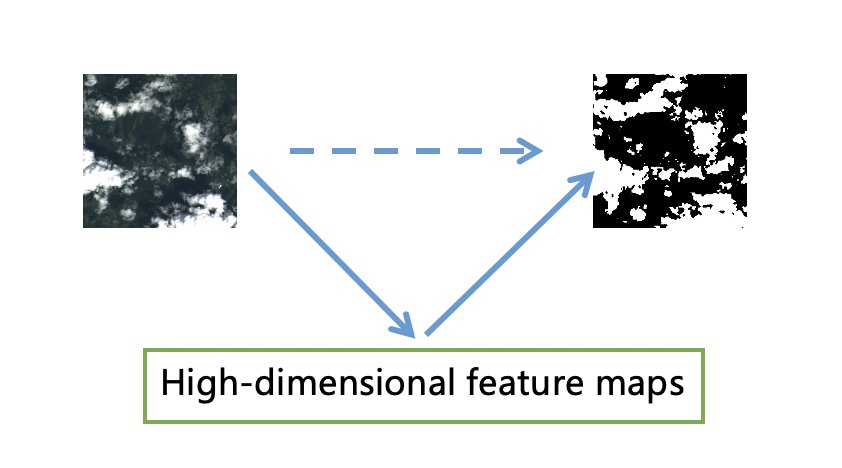
\includegraphics[scale=0.25]{../pic/en-decoder.jpg}
%     \caption{encoder-decoder框架}

%     %英文标题begin
%     \addtocounter{figure}{-1}
%     \vspace{-5pt}
%     %\SetEnglishCaption
%     \renewcommand{\figurename}{Fig}
%     \caption{encoder-decoder framework}
%     \renewcommand{\figurename}{图}
%     %英文标题end
%     \label{fig:en-decoder}
% \end{figure}


目前也有很多方法将全卷积网络应用于遥感图像的云检测。Jeppesena等人\upcite{jeppesen2019cloud}将UNet应用于landsat遥感图像云检测。Chai等人\upcite{chai2019cloud}将SegNet应用于landsat图像。hughes等人\upcite{hughes2019high}将FCN应用于云检测。这些方法都是将光谱与空间特征进行混合提取,很少有人会针对遥感图像多波段的特点对神经网络的结构进行针对性的设计。

卷积神经网络确实可以有效提取图像空间信息,所以应用神经网络做遥感图像的云检测可以表现出较好的性能。但这些方法存在两个缺点:1. 需要大量的参数与昂贵的计算,如UNet有28M个参数。 2.由于混合提取光谱特征与空间特征(我们称之为one-stage),这些模型在保护细节与扩大感受野之间存在着难以调节的矛盾。他们从图像的输入就开始混合像元进行计算,这使得输出的掩膜很难再对单个像素提纯以至于结果非常平滑。

本文提出了一个新颖的、简单的、有效的网络,主要包括两个阶段,模型简略图\ref{fig:spoon_simple}所示。
第一部分,光谱特征提取部分。特征是分类成功的关键,而光谱特征是遥感图像中最本质的特征。在这一部分,我们完全使用1*1的卷积核,不考虑空间信息,对图像进行光谱特征提取。好的光谱特征可以减轻模型的学习压力,使得后续的空间特征更加容易被提取。并且,S-Net将光谱特征提取的结果直达最后的分类层,使得云检测结果更加细腻。
第二部分,空间特征提取部分。这一部分,采用目前主流的空间特征提取框架 --- encoder-decoder框架。不同的是,在这一步,我们不会再重复提取光谱特征,而是采用组卷积(Group Conv)的方式,对第一部分得到的每一种光谱特征作为一组进行单独的卷积。由于第一部分的存在,GC使空间特征提取部分变得廉价且有效。
实验结果表明,S-Net可以在模型参数大大减小的情况下,明显提高云检测精度。
% \end{multicols}

\begin{figure}[H]
    \centering
    \resizebox{\linewidth}{!}{
    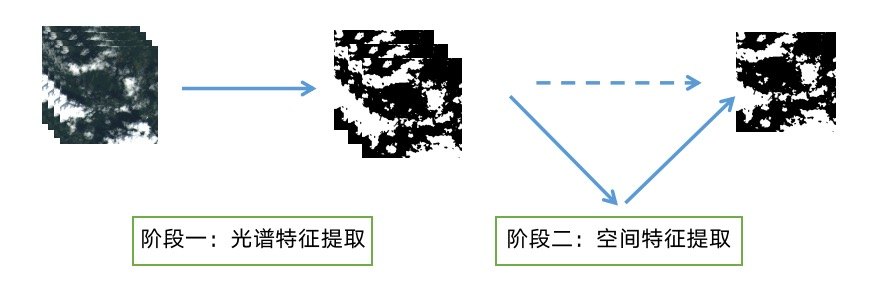
\includegraphics[]{../pic/spoon_simple.jpg}}
    \caption{Spoon-net 框架.}
    %英文标题begin
    \addtocounter{figure}{-1}
    \vspace{-5pt}
    %\SetEnglishCaption
    \renewcommand{\figurename}{Fig}
    \caption{Spoon-net framework}
    \renewcommand{\figurename}{图}
    %英文标题end

    \label{fig:spoon_simple}
\end{figure}

% \begin{multicols}{2} 
\section[]{数据与方法}
\subsection{数据}
本文采用的光学遥感卫星数据集来自NASA landsat8卫星。2013年2月11日,美国航空航天局(NASA) 成功发射Landsat-8卫星。Landsat-8卫星上携带两个传感器,分别是OLI陆地成像仪和TIRS热红外传感器。OLI提供9个波段,波段范围从0.43um到2.30um;TIRS提供地表温度数据,包括两个波段,波段范围从10.60um到12.51um,具体信息见表\ref{landsatBand}。landsat系列卫星每16天可以实现一次全球覆盖。

\begin{table}[H]
    \caption{landsat8波段信息}
    %英文标题begin
    \addtocounter{table}{-1}
    \vspace{-5pt}
    %\SetEnglishCaption
    \renewcommand{\tablename}{Tab}
    \caption{landsat8 band information}
    \renewcommand{\tablename}{表}
    \vspace{5pt}
    %英文标题end

    \centering
    \resizebox{\linewidth}{!}{
    \begin{tabular}{cccc}
    \hline
    传感器类型& 波段 &波长范围($\mu m$)& 空间分辨率\\
    \hline
    \multirow{9}*{OLI}& 1.Coastal& 0.433-0.453& 30\\
    ~&2.Blue& 0.450-0.515& 30\\
    ~&3.Green& 0.525-0.600& 30\\
    ~&4.Red& 0.630-0.680& 30\\
    ~&5.NIR& 0.845-0.885& 30\\
    ~&6.SWIR1& 1.56-1.66& 30\\
    ~&7.SWIR2& 2.1-2.3& 30\\
    ~&8.Pan& 0.5-0.68& 15\\
    ~&9.Cirrus& 1.36-1.39& 30\\
    \hline
    \multirow{2}*{TIRS}& 10.TIRS1& 10.60-11.19& 100\\
    ~& 11.TIRS2& 11.50-12.51& 100\\
    \hline
    \end{tabular}}
    \label{landsatBand}
    \end{table}


为了对模型进行训练与测试,本文利用已有的全球云和云影验证数据集
“L8 Biome Cloud Validation Masks”\upcite{foga2017cloud_data},该数据集共有96景图片,包含8个种类的下垫面。%(including Barren, Forest,Grass/Crops, Shrubland, Snow/Ice, Urban, Water, Wetlands。
% \end{multicols}

% \begin{figure}[H]
%     \centering
%     \includegraphics[scale=0.5]{../pic/BiomeData.png}
%     \caption{Global distribution of the 96 unique Landsat 8 Cloud Cover Assessment (CCA) scenes.}
%     \label{fig:label}
% \end{figure}

% \begin{multicols}{2} 
每景图片的标签均是人工标注,可信度较高。每个文件包含.TIF格式的Landsat 8 Level-1数据文件、质量文件和.img(ENVI)格式的真值标签,人工标志位如表\ref{BiomeFlag}所示。

\begin{table}[H]
    \caption{L8 Biome 数据人工标注标志位}
    %英文标题begin
    \addtocounter{table}{-1}
    \vspace{-5pt}
    %\SetEnglishCaption
    \renewcommand{\tablename}{Tab}
    \caption{flag of landsat8 biome}
    \renewcommand{\tablename}{表}
    \vspace{5pt}
    %英文标题end

    \centering
    \resizebox{\linewidth}{!}{
    \begin{tabular}{cccccc}
    \hline
    value& 0& 64& 128& 192& 255\\
    \hline
    Interpretation&	Fill& Cloud Shadow& Clear &Thin Cloud& Cloud\\
    \hline
    \end{tabular}}
    
    \label{BiomeFlag}
    \end{table}

根据云量百分比的多少,‘L8 Biome’中96景分为clear, midcloud, cloud三种,每种各占三分之一,云量低于35\%的为clear,云量高于65\%的为cloud,云量介于35\%与65\%之间的为midcloud。本文使用midcloud的所有数据,共32景做实验,每种地物有4景。数据我们将标签简单地分为云与非云两类,将每景L8图像均匀切割为256*256大小的小图,切割时过滤掉带填充值的图片,因此,图像边缘的填充像素并不会出现在训练与测试的步骤中。波段选择了除了全色波段的所有波段,共10个波段,训练集与测试集的比例为6:4,训练集有10247张子图,测试集有6932张子图。

\subsection{网络结构}

S-Net是一个两阶段模型,将光谱特征提取与空间特征提取解藕,第一阶段是光谱特征提取阶段,第二阶段是空间特征提取阶段,详细模型结构如图\ref{fig_myModel}所示。
\end{multicols}

\begin{figure}[H]
    \centering
    \resizebox{\linewidth}{!}{
    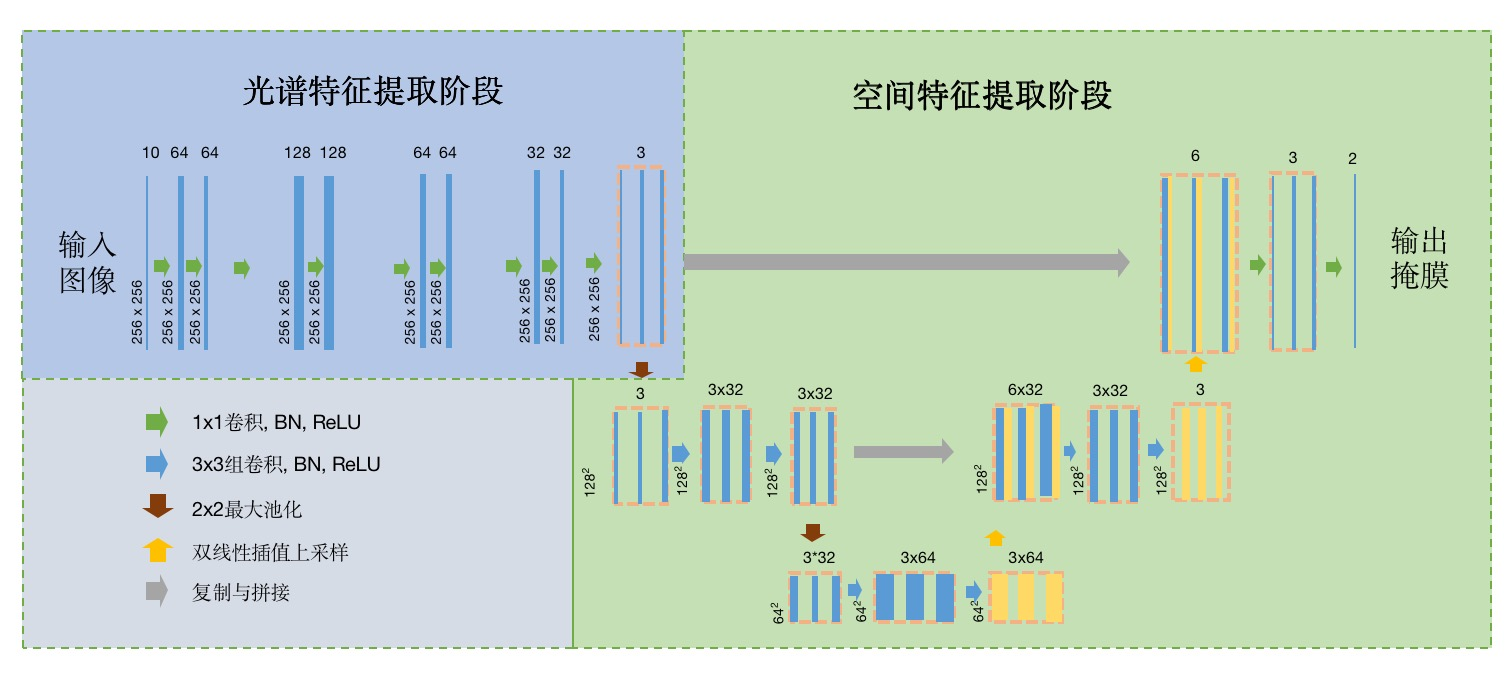
\includegraphics[scale=1]{../pic/spoon.jpg}}
    \caption{Spoon-net 详细结构.}
    %英文标题begin
    \addtocounter{figure}{-1}
    \vspace{-5pt}
    %\SetEnglishCaption
    \renewcommand{\figurename}{Fig}
    \caption{Spoon-net framework}
    \renewcommand{\figurename}{图}
    %英文标题end
    \label{fig_myModel}
\end{figure}
\begin{multicols}{2} 
1. 光谱特征提取阶段。 该阶段使用1*1的卷积核对单个像素进行计算,不涉及到空间信息,可以有效保持图像的细节。多层1*1的卷积操作等价于一个多层感知机(MLP),MLP可以有效提取非线性光谱特征,为后续分类提供良好的基础,并且不会降低图像分辨率。这一阶段输出的每一层特征图都是一种有效的光谱特征,类似于NDVI、NDWI等,但远比它们复杂得多,更加具有非线性,也更有效。详细结构如图\ref{pic:straight}所示。

\begin{figure}[H]
    \centering
    \resizebox{\linewidth}{!}{
    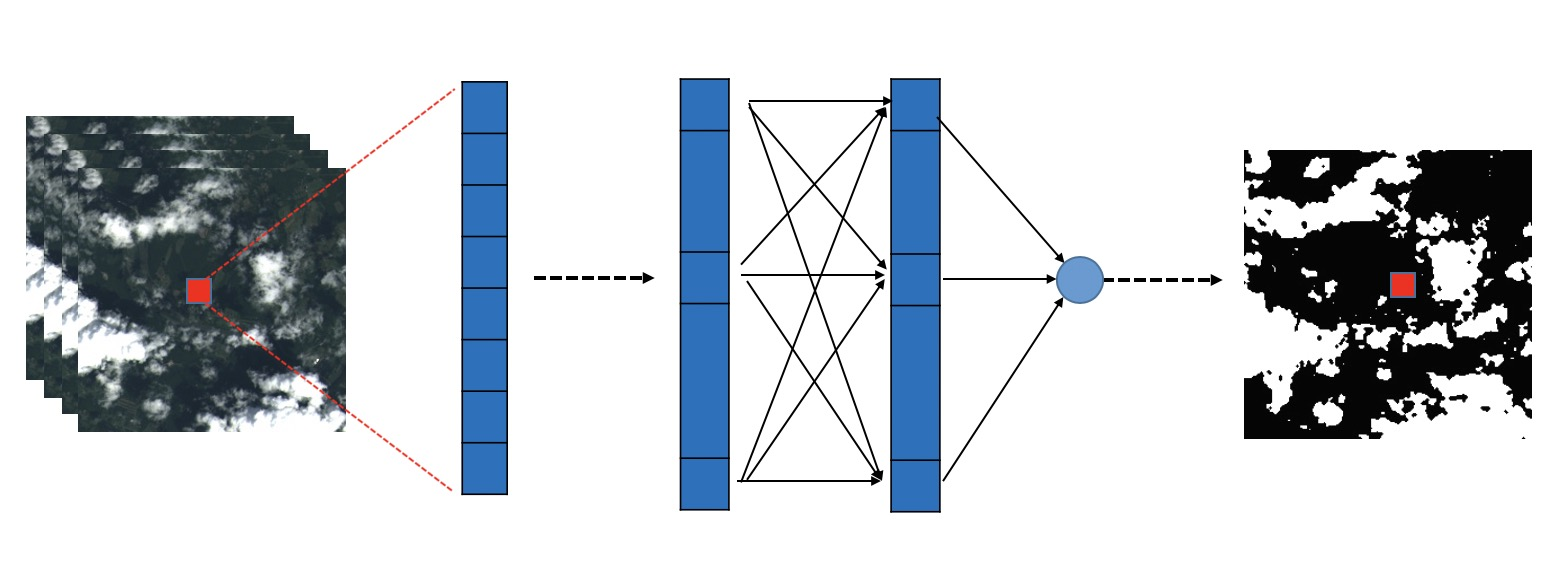
\includegraphics[scale=1]{../pic/part1.jpg}}
    \caption[]{阶段一: 所有的卷积核都是1*1大小的,等价于多层感知机。}
    %英文标题begin
    \addtocounter{figure}{-1}
    \vspace{-5pt}
    %\SetEnglishCaption
    \renewcommand{\figurename}{Fig}
    \caption{stage 1: all convolutional kernels are 1 * 1, which is equivalent to multi-layer perceptron.}
    \renewcommand{\figurename}{图}
    %英文标题end
    \label{pic:straight}
\end{figure}

这一阶段生成的光谱特征,不仅会用于第二阶段的空间特征提取,还会以跳层连接的方式直接参与最终的分类,并且分类层的卷积核也是1*1,这意味着我们的网络有足够的能力保证分割结果的细节。实验发现,当光谱特征数为3时,具有最高的分类精度与f1值。

\begin{table}[H]
    \caption{光谱特征提取层数对实验结果的影响}
    %英文标题begin
    \addtocounter{table}{-1}
    \vspace{-5pt}
    %\SetEnglishCaption
    \renewcommand{\tablename}{Tab}
    \caption{Influence of the number of spectral feature extraction layers on experimental results}
    \renewcommand{\tablename}{表}
    \vspace{5pt}
    %英文标题end

    \centering
    \resizebox{\linewidth}{!}{
    \begin{tabular}{cccc}
    \hline
    光谱层数& acc& f1& 参数数量\\
    \hline
    2&	94.38&  94.11& 238K\\
    3&  \textbf{95.34}&  \textbf{95.05}& 342K\\
    4&  94.79&  94.46& 450K\\
    5&  94.92&  94.60& 562K\\
    6&  94.84&  94.61& 678K\\
    \hline
    \end{tabular}}
    
    \label{BiomeFlag}
    \end{table}

2. 空间信息提取阶段。光谱特征虽然可以保持分辨率、解析细节,但它们不包含特定区域的信息与上下文信息,容易造成较高的虚警率,因此我们仍需要提取空间信息去优化。

encoder-decoder结构是图像分割领域常用的一种空间信息提取结构,它通过多层卷积与下采样层提取大感受野内的空间信息,通过多层卷积与上采样层将特征图还原到原始分辨率。丰富的空间信息需要更多的下采样层和更大的感受野,但随之而来的问题是越来越容易忽略细节,因此encoder-decoder结构加入了跳层连接,将高分辨率的特征图与低分辨率的空间信息结合,以缓和这一矛盾。
图\ref{pic:part2}展示了每一组光谱特征的卷积过程。

\begin{figure}[H]
    \centering
    \resizebox{\linewidth}{!}{
    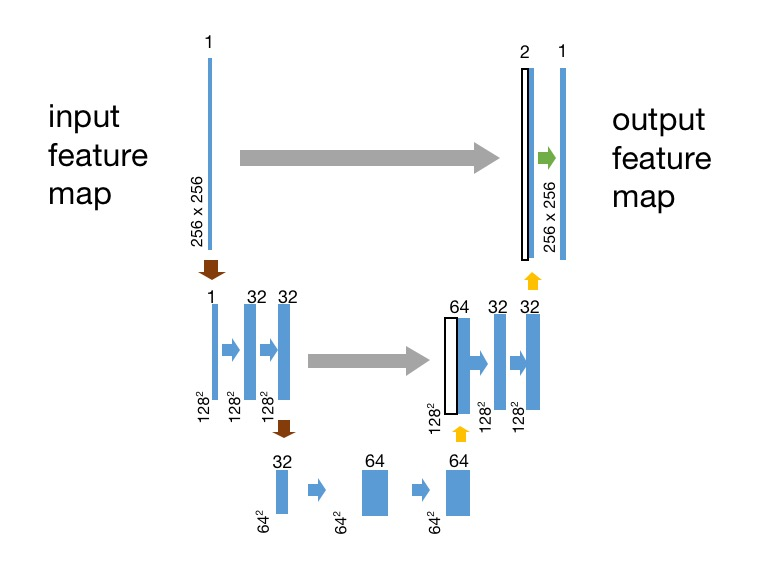
\includegraphics[scale=1]{../pic/groupcov.jpg}}
    \caption[]{阶段二: 每组特征图的卷积过程。}
    %英文标题begin
    \addtocounter{figure}{-1}
    \vspace{-5pt}
    %\SetEnglishCaption
    \renewcommand{\figurename}{Fig}
    \caption{stage 2: Convolution process of each group.}
    \renewcommand{\figurename}{图}
    %英文标题end
    \label{pic:part2}
\end{figure}

为了更加有效提取空间信息,避免在光谱上的重复计算,我们引入组卷积的概念。图\ref{pic:GC}展示了组卷积与普通卷积的区别。通过光谱特征提取阶段我们已经得到非常有效的光谱特征,我们在这一部分不会再重复地计算光谱特征,我们对每一种光谱特征进行单独的、相同的编码解码,并将每一个光谱特征的卷积结果作为一组,进行下采样、上采样等操作。组卷积的优势在于可以专注于提取空间信息,免受光谱信息的交互与干扰,并且节省了大量参数与电脑计算力(组卷积使网络的参数与计算量减小为原来的三分之一),减少了模型过拟合的风险。

\begin{figure}[H]
    \centering
    \resizebox{0.9\linewidth}{!}{
    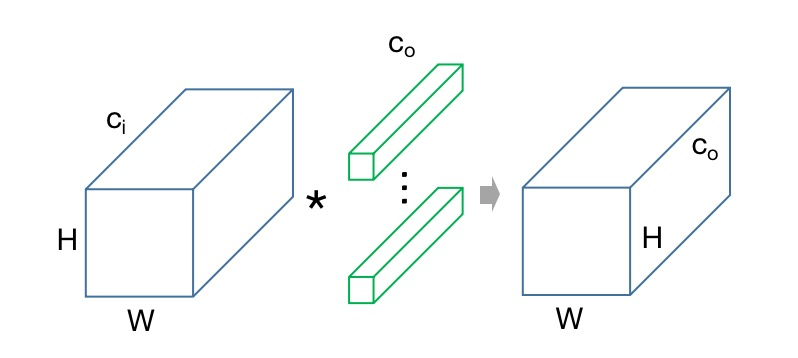
\includegraphics[scale=1]{../pic/conv.jpg}}
    \caption[]{组卷积与普通卷积的区别。}
    %英文标题begin
    \addtocounter{figure}{-1}
    \vspace{-5pt}
    %\SetEnglishCaption
    \renewcommand{\figurename}{Fig}
    \caption{The difference between group convolution and ordinary convolution}
    \renewcommand{\figurename}{图}
    %英文标题end
    \label{pic:GC}
\end{figure}

同时,我们也了减少encoder-decoder层数。由于光谱特征提取部分的存在,在这一部分模型提取空间信息的压力已经被大大减小,所以我们并不需要很深的网络、很多的参数去拟合很复杂的空间特征,因此我们可以大胆减少encoder-decoder层数,而随着层数的减少,参数量几乎是几何减少的。实验发现,当encoder-decoder层数大于2时,云检测效果不会再有提高。

\begin{table}[H]
    \caption{光谱特征提取层数对实验结果的影响}
    %英文标题begin
    \addtocounter{table}{-1}
    \vspace{-5pt}
    %\SetEnglishCaption
    \renewcommand{\tablename}{Tab}
    \caption{Influence of the number of spectral feature extraction layers on experimental results}
    \renewcommand{\tablename}{表}
    \vspace{5pt}
    %英文标题end

    \centering
    \resizebox{0.9\linewidth}{14mm}{
    \begin{tabular}{cccc}
    \hline
    下采样层数& acc& f1& 参数数量\\
    \hline
    1&	92.33&  92.12& 72K\\
    2&  \textbf{95.34}&  \textbf{95.05}& 341K\\
    3&  95.01&  94.89& 1.4M\\
    4&  94.87&  94.62& 5.7M\\
    \hline
    \end{tabular}}
    
    \label{BiomeFlag}
    \end{table}

上采样的方式一般有四种:插值法,反卷积,反池化,超分辨率重建领域的亚像素卷积插值。双线性插值是目前在语义分割中用的比较多的一种插值方式,比如FCN中就是用的这种方法。在CNN上下文中,反卷积是卷积的逆过程,卷积用于提取空间信息,反卷积用于解析空间信息。在实现上,反卷积是卷积的转置,所以反卷积也叫做转置卷积。反池化是池化的逆过程,在池化过程中,记录下max-pooling在对应kernel中的坐标,在反池化过程中,将一个元素根据kernel进行放大,根据之前的坐标将元素填写进去,其他位置补0 。在下采样的时候记录max的位置,上采样的时候最大值的位置还原,其它位置填0。反池化是速度最快的上采样操作,计算量和参数也特别少,但是准确率一般。虽然理论上,由于反卷积具有更多的参数,所以反卷积可以更好的学习特征,但是有研究表明,如果参数配置不当,反卷积很容易出现输出feature map带有明显棋盘状的现象\upcite{odena2016deconvolution},双线性差值可以取得与反卷积相同甚至更好的效果。因此,我们选择参数少且容易取得较好效果的双线性差值法。


在卷积之后,激活函数之前,一般会有一个批归一化操作\upcite{ioffe2015batch}(Batch Normalization)。BN是一种非常优雅的重参数化的方法,它的存在类似于为网络中不同的层设置了不同的学习率。为神经网络输入的多个数据称为batch,BN以batch为单位,先将上一层网络的输出在通道上标准化为标准正态分布,再进行缩放与平移操作,可以将上一层的输出调整在一个较好的范围内,结果就是模型训练更加容易。

\begin{equation}
    BN(x) = \gamma\frac{x-\mu}{\sigma}+\beta
\end{equation}

本文中几乎所有的激活函数都是ReLU函数,$\sigma(x)=max(0,x)$。ReLU函数是一种分段线性函数,把所有的负值都变为0,而正值不变,这种操作被成为单侧抑制。单侧抑制使得神经网络中的神经元也具有了稀疏激活性。我们认为对于某种地物可以对某个特殊的指标有响应,而对其他指标就反应一般。所以ReLU实现稀疏后的模型能够更好地挖掘相关特征,且ReLU由于非负区间的梯度为常数,因此不存在梯度消失问题,使得模型的收敛速度维持在一个稳定状态。

\begin{equation}
    ReLU(x)=\left\{
    \begin{aligned}
        x, & &\text{if} & & x > 0 \\
        0, & &\text{if} & & x \leq 0
    \end{aligned}
    \right.
\end{equation}

在最后一层卷积层,激活函数会使用sigmoid函数,用于将输出映射到0-1之间,代表该像素点为云的概率。为了训练模型,使用交叉熵损失函数计算损失,并用带动量的随即梯度下降法进行训练。
\begin{equation}
    L = -\sum_{i=1}^N y_ilog(\hat{y}_i)+(1-y_i)log(1-\hat{y}_i)
\end{equation}
其中,$N$表示所有所有样本个数,$y_i$代表标签真值,$\hat{y_i}$代表模型预测值。

\section[]{实验与结果}

为客观评定算法的有效性和优越性,采用准确率,召回率,精确度,$F_1$值对结果进行评估。其中,准确率衡量像素分类正确的概率;召回率衡量属于云的像素中被分类正确的概率,是漏警率的相反数;精确度衡量被识别为云的像素中真正是云的概率,是虚警率的相反数;$F_1$值是召回率与精确度的调和平均数,常被用于二分类问题,可以有效衡量样本不均衡时检测结果的好坏。四个评价指标分别为:

\begin{equation}
    A = \frac{TP + TN}{TP + TN + FP + FN}\label{acc}
\end{equation}
\begin{equation}
    R = \frac{TP}{TP + FN}\label{recall}
\end{equation}
\begin{equation}
    P = \frac{TP}{TP + FP}\label{precision}
\end{equation}
\begin{equation}
    F = \frac{2 * R_{recall} * R_{precision}}{R_{recall} + R_{precision}}\label{f1}
\end{equation}

其中,TP为真正类(True Positive),即云被判为云;TN为真负类(True Negative),即非云被判为非云;FP为假正类(False Positive),即非云被判为云;FN为假负类(false Negative),云被判为非云。

本文将模型与CFMask、原始的UNet做比较。输入是除了全色波段的其余10个波段,将所有图像按6:4随机划分为训练集和测试集,并调整UNet的输入通道数为10。将ground truth分为云与非云两类。有研究表明\upcite{chai2019cloud}输入DN值(Digital number)或大气顶部反射率(ToA)数据,会取得相似的结果,我们选择使用DN值作为模型输入,并为了使训练更加稳定,对输入进行归一化。
具体参数,如学习率为$1e^{-2}$,批训练大小为 8,采用动量为0.9的随即梯度下降法训练。我们的损失函数包括两部分,分别计算光谱与空间特征提取两阶段的损失,如图\ref{pic:loss}所示。为了使模型更加容易收敛,auxiliary loss的权重逐渐降低,final loss的权重逐渐增高,分为3个阶段:(0.8, 0.2)、(0.2, 0.8)、(0, 1)。

\begin{figure}[H]
    \centering
    \resizebox{\linewidth}{!}{
    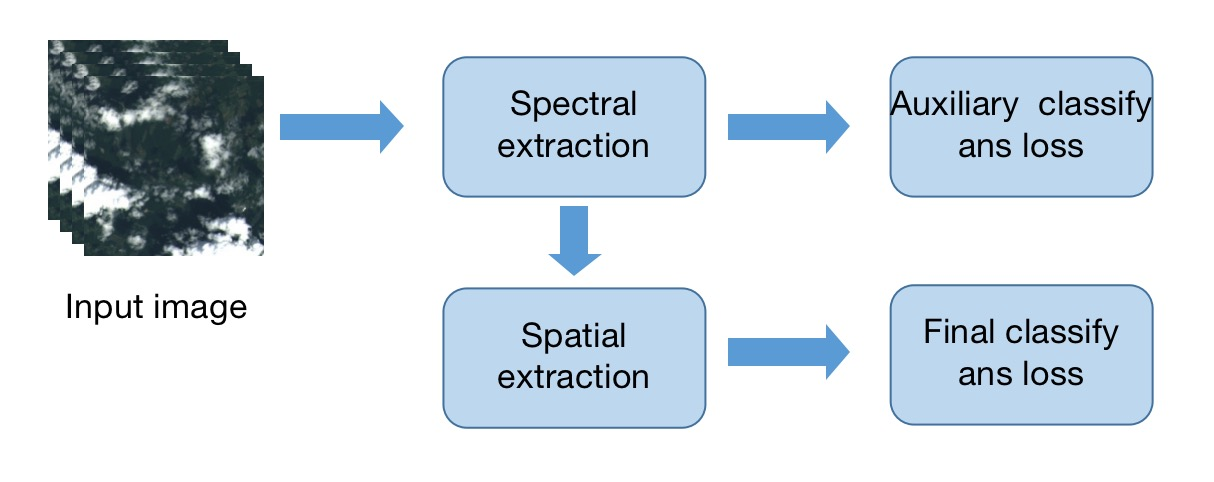
\includegraphics[scale=1]{../pic/loss.jpg}}
    \caption[]{两个损失函数。}
    %英文标题begin
    \addtocounter{figure}{-1}
    \vspace{-5pt}
    %\SetEnglishCaption
    \renewcommand{\figurename}{Fig}
    \caption{Two loss function}
    \renewcommand{\figurename}{图}
    %英文标题end
    \label{pic:loss}
\end{figure}

如表(\ref{tab_eval})所示,相比于CFMask,取得了8个百分点的性能提升;在模型参数量只有unet的八十分之一的情况下,准确率和f1值均高于unet,更加轻量,具有更大的应用潜力。所有实验均在Ubuntu 16.04的Pytorch上进行,处理器为Nvidia titan xp, 内存16 GB。
\end{multicols}

\begin{table}[H]
    \caption{实验结果对比}
    %英文标题begin
    \addtocounter{table}{-1}
    \vspace{-5pt}
    %\SetEnglishCaption
    \renewcommand{\figurename}{Tab}
    \caption{Comparison of experimental results}
    \vspace{5pt}
    \renewcommand{\figurename}{表}
    %英文标题end
    \centering
    \resizebox{0.9\textwidth}{!}{
    \begin{tabular}{c|cccccccccc}
        \hline
        model& evaluation& Barren& Forest& Grass/Crops& Shrubland& Snow/Ice& Urban& Water&  Wetlands& total\\
        \hline
        \multirow{4}*{SpoonNet-3}
        &acc   &96.43 &96.61 &94.48 &95.08 &96.29 &94.85 &94.38 &94.56 &\textbf{95.34}\\
        &rec.  &96.46 &95.90 &92.67 &93.21 &95.38 &97.07 &91.90 &98.60 &\textbf{95.15}\\
        &prec. &97.89 &99.38 &93.10 &97.41 &95.61 &91.57 &92.82 &92.34 &95.01\\
        &F1    &97.17 &97.61 &92.89 &95.26 &95.50 &94.24 &92.36 &95.37 &\textbf{95.05}\\
        \hline
        \multirow{4}*{U-Net}
        &acc   &96.09 &94.51 &92.67 &94.48 &91.78 &95.00 &93.74 &94.90 &94.15\\
        &rec.  &96.00 &92.96 &81.91 &91.58 &89.16 &96.22 &89.83 &98.34 &92.00\\
        &prec. &97.60 &99.22 &97.31 &97.77 &90.90 &92.56 &93.97 &93.05 &\textbf{95.30}\\
        &F1    &96.80 &95.99 &88.95 &94.58 &90.02 &94.36 &91.85 &95.62 &93.52\\
        \hline
        \multirow{4}*{CFMask}
        &acc   &87.46 &95.20 &85.42 &90.34 &60.97 &83.05 &91.51 &90.78 &86.09\\
        &rec.  &90.85 &93.87 &68.03 &92.04 &92.21 &96.07 &92.22 &96.37 &91.45\\
        &prec. &88.99 &99.31 &88.85 &89.83 &51.74 &73.25 &86.97 &88.38 &82.89\\
        &F1    &89.91 &96.51 &77.05 &90.92 &66.29 &83.13 &89.52 &92.21 &86.96\\
        \hline
    \end{tabular}}
    
    \label{tab_eval}
\end{table}

\begin{multicols}{2}

相比于一阶段的UNet,我们的模型具有更高的准确率与f1值,准确率达到95.34\%,而UNet只有94.15\%,比UNet高了一个百分点;f1值有0.9505,而UNet只有0.9352,比UNet高了1.5个百分点。同时可以发现,我们的模型对于碎云、细节有良好的检测与保持能力。unet的识别更加光滑,使得一些细节被忽略,而我们的模型更加注重细节,这对于云检测是一个很重要的能力。如图\ref{Fig.main1}所示,从左到右依次为真彩色图、人工标注、光谱特征提取结果构成的假彩色图、我们的模型预测结果、UNet结果,白色代表云,黑色代表非云,第二行是第一行黄色方框的放大图,以此类推。我们的模型由于有光谱特征提取层的存在,并且光谱特征直达最后的分类层,所以对细节有较好的保持,对碎云有良好的识别,能以极少的参数在整体上达到优于U-Net的效果。

\begin{figure}[H]
    \centering
    \subfigure[Color]{
        \begin{minipage}[b]{0.15\linewidth}
            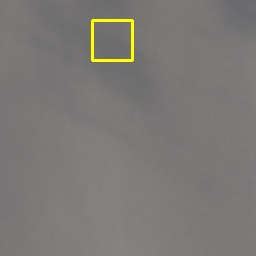
\includegraphics[width=1\linewidth]{../log/spoon2/cut/LC81321192014054LGN00_03055_color.jpg}\vspace{4pt}
            
\includegraphics[width=1\linewidth]{../log/spoon2/cut/tmp_cut_LC81321192014054LGN00_03055_color.jpg}\vspace{4pt}
            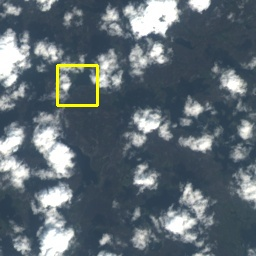
\includegraphics[width=1\linewidth]{../log/spoon2/cut/LC80350192014190LGN00_06561_color.jpg}\vspace{4pt}
            
\includegraphics[width=1\linewidth]{../log/spoon2/cut/tmp_cut_LC80350192014190LGN00_06561_color.jpg}\vspace{4pt}
            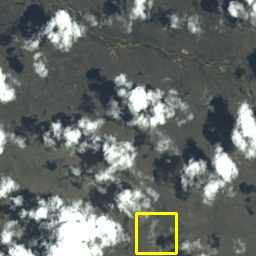
\includegraphics[width=1\linewidth]{../log/spoon2/cut/LC80980712014024LGN00_15443_color.jpg}\vspace{4pt}
            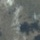
\includegraphics[width=1\linewidth]{../log/spoon2/cut/tmp_cut_LC80980712014024LGN00_15443_color.jpg}\vspace{4pt}
        \end{minipage}
    }
    \subfigure[GT]{
        \begin{minipage}[b]{0.15\linewidth}
            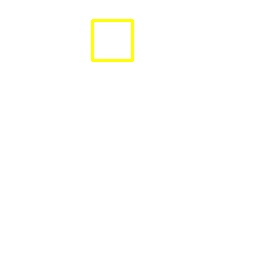
\includegraphics[width=1\linewidth]{../log/spoon2/cut/LC81321192014054LGN00_03055_mask.jpg}\vspace{4pt}
            
\includegraphics[width=1\linewidth]{../log/spoon2/cut/tmp_cut_LC81321192014054LGN00_03055_mask.jpg}\vspace{4pt}
            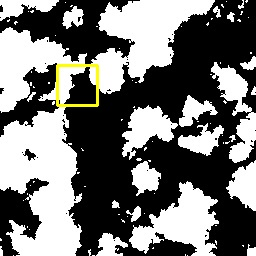
\includegraphics[width=1\linewidth]{../log/spoon2/cut/LC80350192014190LGN00_06561_mask.jpg}\vspace{4pt}
            
\includegraphics[width=1\linewidth]{../log/spoon2/cut/tmp_cut_LC80350192014190LGN00_06561_mask.jpg}\vspace{4pt}
            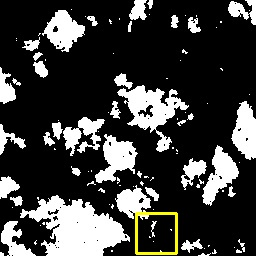
\includegraphics[width=1\linewidth]{../log/spoon2/cut/LC80980712014024LGN00_15443_mask.jpg}\vspace{4pt}
            
\includegraphics[width=1\linewidth]{../log/spoon2/cut/tmp_cut_LC80980712014024LGN00_15443_mask.jpg}\vspace{4pt}
        \end{minipage}
    }
    \subfigure[Spectral]{
        \begin{minipage}[b]{0.15\linewidth}
            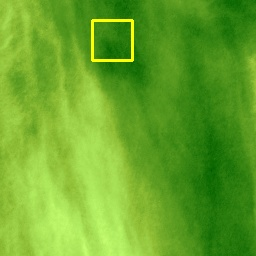
\includegraphics[width=1\linewidth]{../log/spoon2/cut/LC81321192014054LGN00_03055_spectral.jpg}\vspace{4pt}
            
\includegraphics[width=1\linewidth]{../log/spoon2/cut/tmp_cut_LC81321192014054LGN00_03055_spectral.jpg}\vspace{4pt}
            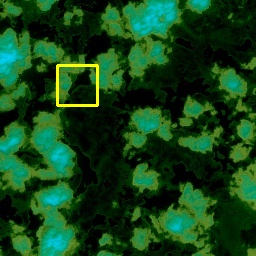
\includegraphics[width=1\linewidth]{../log/spoon2/cut/LC80350192014190LGN00_06561_spectral.jpg}\vspace{4pt}
            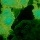
\includegraphics[width=1\linewidth]{../log/spoon2/cut/tmp_cut_LC80350192014190LGN00_06561_spectral.jpg}\vspace{4pt}
            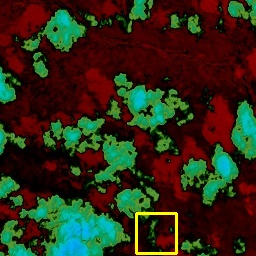
\includegraphics[width=1\linewidth]{../log/spoon2/cut/LC80980712014024LGN00_15443_spectral.jpg}\vspace{4pt}
            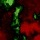
\includegraphics[width=1\linewidth]{../log/spoon2/cut/tmp_cut_LC80980712014024LGN00_15443_spectral.jpg}\vspace{4pt}
        \end{minipage}
    }
    \subfigure[SNet]{
        \begin{minipage}[b]{0.15\linewidth}
            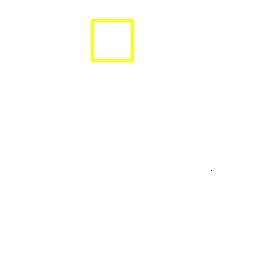
\includegraphics[width=1\linewidth]{../log/spoon2/cut/LC81321192014054LGN00_03055_my.jpg}\vspace{4pt}
            
\includegraphics[width=1\linewidth]{../log/spoon2/cut/tmp_cut_LC81321192014054LGN00_03055_my.jpg}\vspace{4pt}
            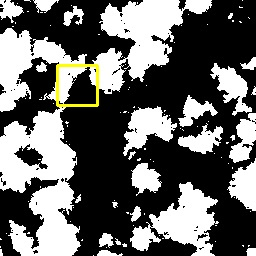
\includegraphics[width=1\linewidth]{../log/spoon2/cut/LC80350192014190LGN00_06561_my.jpg}\vspace{4pt}
            
\includegraphics[width=1\linewidth]{../log/spoon2/cut/tmp_cut_LC80350192014190LGN00_06561_my.jpg}\vspace{4pt}
            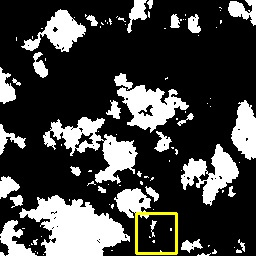
\includegraphics[width=1\linewidth]{../log/spoon2/cut/LC80980712014024LGN00_15443_my.jpg}\vspace{4pt}
            
\includegraphics[width=1\linewidth]{../log/spoon2/cut/tmp_cut_LC80980712014024LGN00_15443_my.jpg}\vspace{4pt}
        \end{minipage}
    }
    \subfigure[UNet]{
        \begin{minipage}[b]{0.15\linewidth}
            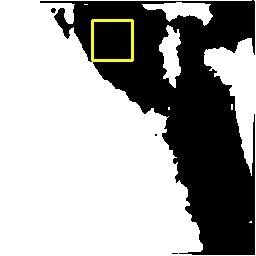
\includegraphics[width=1\linewidth]{../log/spoon2/cut/LC81321192014054LGN00_03055_unet.jpg}\vspace{4pt}
            
\includegraphics[width=1\linewidth]{../log/spoon2/cut/tmp_cut_LC81321192014054LGN00_03055_unet.jpg}\vspace{4pt}
            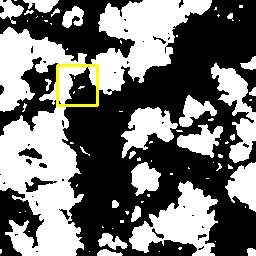
\includegraphics[width=1\linewidth]{../log/spoon2/cut/LC80350192014190LGN00_06561_unet.jpg}\vspace{4pt}
            
\includegraphics[width=1\linewidth]{../log/spoon2/cut/tmp_cut_LC80350192014190LGN00_06561_unet.jpg}\vspace{4pt}
            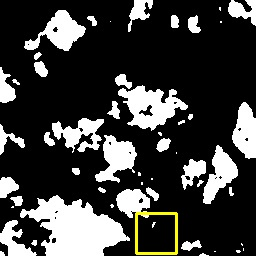
\includegraphics[width=1\linewidth]{../log/spoon2/cut/LC80980712014024LGN00_15443_unet.jpg}\vspace{4pt}
            
\includegraphics[width=1\linewidth]{../log/spoon2/cut/tmp_cut_LC80980712014024LGN00_15443_unet.jpg}\vspace{4pt}
        \end{minipage}
    }
\caption{Spoon-Net检测结果展示}
%英文标题begin
\addtocounter{figure}{-1}
\vspace{-5pt}
%\SetEnglishCaption
\renewcommand{\figurename}{Fig}
\caption{Example of spoon-net results}
\renewcommand{\figurename}{图}
%英文标题end
\label{Fig.main1}
\end{figure}

我们的模型参数量有0.34M,而主流网络如U-Net有28M,FCN有20.5M。其他网络参数多的主要原因是具有更深的encoder-decoder结构,以U-Net为例,U-Net最深一层就有14M的参数,占据了所有参数的一半。
我们的模型由于更加注重单个像素的光谱特征,在提取空间信息之前先使用少量的参数(1*1卷积核)提取光谱信息,使得我们可以大胆的减少encoder-decoder层数,同时引入组卷积的操作,极大地简化模型,大大降低参数量。

% \begin{table}[H]
%     \centering
%     \resizebox{\textwidth}{!}{
%     \begin{tabular}{c|cccccccccc}
%         \hline
%         \hline
%         model& evaluation& Barren& Forest& Grass/Crops& Shrubland& Snow/Ice& Urban& Water&  Wetlands& total\\
%         \hline
%         \multirow{4}*{S-Net}
%         &rec.  &5.54 &50.49 &25.13 &31.62 &6.21 &31.11 &28.15 &25.77 &25.50\\
%         &prec. &6.89 &50.10 &26.27 &32.82 &2.98 &18.65 &21.81 &30.42 &23.74\\
%         &F1    &6.14 &50.30 &25.69 &32.21 &4.03 &23.32 &24.58 &27.90 &24.27\\
%         \hline
%         \multirow{4}*{U-Net}
%         &rec.  &14.23 &20.88 &25.69 &23.24 &6.02 &27.66 &16.72 &27.10 &20.19\\
%         &prec. &24.52 &29.39 &37.55 &32.66 &3.33 &27.08 &19.52 &42.50 &27.07\\
%         &F1    &18.01 &24.42 &30.51 &27.16 &4.29 &27.37 &18.01 &33.10 &22.86\\
%         \hline
%         \multirow{4}*{CFMask}
%         &rec.  &8.80 &56.97 &23.26 &23.65 &4.33 &22.62 &28.21 &19.00 &23.36\\
%         &prec. &3.60 &47.16 &16.09 &12.41 &0.50 &12.81 &8.48 &12.58 &14.20\\
%         &F1    &5.11 &51.60 &19.02 &16.28 &0.89 &16.35 &13.04 &15.14 &17.18\\
%         \hline
%         \hline
%     \end{tabular}}
%     \caption{Evaluation results on the Biome dataset}
%     \label{tab_eval}
% \end{table}

而且,有研究表明\upcite{scaramuzza2011development}人工标注的数据可能存在7\%左右的错误。尤其对于一些碎云、半透明的薄云,评判标准可能会因人而异。我们发现,'L8 Biome'数据确实存在一些问题。同时,由于人工标注的不稳定性,简单地依靠评价指标可能并不能真实反应模型的优劣,因为大部分模型都很容易对于大面积的厚云(低下垫面信息的)有较好的识别能力;并且以这些标签为真值进行的训练,可能也会存在问题。

\begin{figure}[H]
    \centering
    \subfigure[Color]{
        \begin{minipage}[b]{0.15\linewidth}
            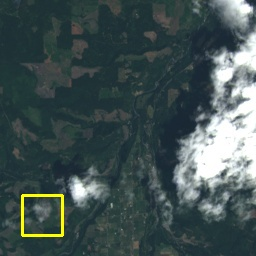
\includegraphics[width=1\linewidth]{../log/spoon2/cut2/LC80460282014171LGN00_12434_color.jpg}\vspace{4pt}
            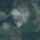
\includegraphics[width=1\linewidth]{../log/spoon2/cut2/tmp_cut_LC80460282014171LGN00_12434_color.jpg}\vspace{4pt}
            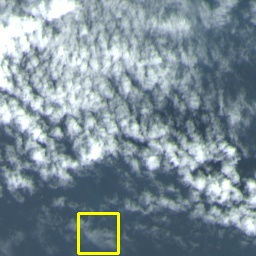
\includegraphics[width=1\linewidth]{../log/spoon2/cut2/LC81620432014072LGN00_16237_color.jpg}\vspace{4pt}
            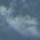
\includegraphics[width=1\linewidth]{../log/spoon2/cut2/tmp_cut_LC81620432014072LGN00_16237_color.jpg}\vspace{4pt}
            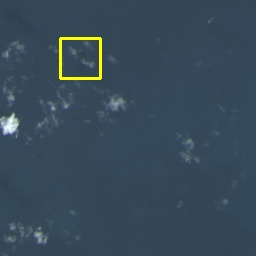
\includegraphics[width=1\linewidth]{../log/spoon2/cut2/LC81620432014072LGN00_16329_color.jpg}\vspace{4pt}
            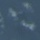
\includegraphics[width=1\linewidth]{../log/spoon2/cut2/tmp_cut_LC81620432014072LGN00_16329_color.jpg}\vspace{4pt}
        \end{minipage}
    }
    \subfigure[GT]{
        \begin{minipage}[b]{0.15\linewidth}
            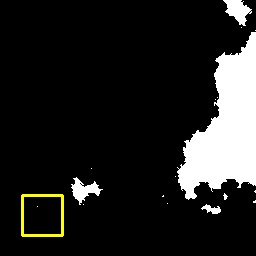
\includegraphics[width=1\linewidth]{../log/spoon2/cut2/LC80460282014171LGN00_12434_mask.jpg}\vspace{4pt}
            
\includegraphics[width=1\linewidth]{../log/spoon2/cut2/tmp_cut_LC80460282014171LGN00_12434_mask.jpg}\vspace{4pt}
            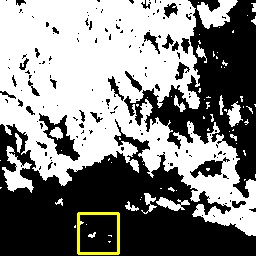
\includegraphics[width=1\linewidth]{../log/spoon2/cut2/LC81620432014072LGN00_16237_mask.jpg}\vspace{4pt}
            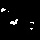
\includegraphics[width=1\linewidth]{../log/spoon2/cut2/tmp_cut_LC81620432014072LGN00_16237_mask.jpg}\vspace{4pt}
            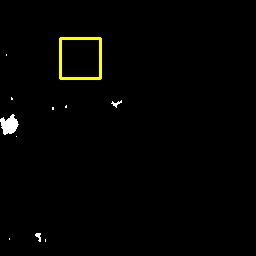
\includegraphics[width=1\linewidth]{../log/spoon2/cut2/LC81620432014072LGN00_16329_mask.jpg}\vspace{4pt}
            
\includegraphics[width=1\linewidth]{../log/spoon2/cut2/tmp_cut_LC81620432014072LGN00_16329_mask.jpg}\vspace{4pt}
        \end{minipage}
    }
    \subfigure[Spectral]{
        \begin{minipage}[b]{0.15\linewidth}
            \includegraphics[width=1\linewidth]{../log/spoon2/cut2/LC80460282014171LGN00_12434_spectral.jpg}\vspace{4pt}
            \includegraphics[width=1\linewidth]{../log/spoon2/cut2/tmp_cut_LC80460282014171LGN00_12434_spectral.jpg}\vspace{4pt}
            \includegraphics[width=1\linewidth]{../log/spoon2/cut2/LC81620432014072LGN00_16237_spectral.jpg}\vspace{4pt}
            \includegraphics[width=1\linewidth]{../log/spoon2/cut2/tmp_cut_LC81620432014072LGN00_16237_spectral.jpg}\vspace{4pt}
            \includegraphics[width=1\linewidth]{../log/spoon2/cut2/LC81620432014072LGN00_16329_spectral.jpg}\vspace{4pt}
            \includegraphics[width=1\linewidth]{../log/spoon2/cut2/tmp_cut_LC81620432014072LGN00_16329_spectral.jpg}\vspace{4pt}
        \end{minipage}
    }
    \subfigure[SNet]{
        \begin{minipage}[b]{0.15\linewidth}
            \includegraphics[width=1\linewidth]{../log/spoon2/cut2/LC80460282014171LGN00_12434_my.jpg}\vspace{4pt}
            \includegraphics[width=1\linewidth]{../log/spoon2/cut2/tmp_cut_LC80460282014171LGN00_12434_my.jpg}\vspace{4pt}
            \includegraphics[width=1\linewidth]{../log/spoon2/cut2/LC81620432014072LGN00_16237_my.jpg}\vspace{4pt}
            \includegraphics[width=1\linewidth]{../log/spoon2/cut2/tmp_cut_LC81620432014072LGN00_16237_my.jpg}\vspace{4pt}
            \includegraphics[width=1\linewidth]{../log/spoon2/cut2/LC81620432014072LGN00_16329_my.jpg}\vspace{4pt}
            \includegraphics[width=1\linewidth]{../log/spoon2/cut2/tmp_cut_LC81620432014072LGN00_16329_my.jpg}\vspace{4pt}
        \end{minipage}
    }
    \subfigure[UNet]{
        \begin{minipage}[b]{0.15\linewidth}
            \includegraphics[width=1\linewidth]{../log/spoon2/cut2/LC80460282014171LGN00_12434_unet.jpg}\vspace{4pt}
            \includegraphics[width=1\linewidth]{../log/spoon2/cut2/tmp_cut_LC80460282014171LGN00_12434_unet.jpg}\vspace{4pt}
            \includegraphics[width=1\linewidth]{../log/spoon2/cut2/LC81620432014072LGN00_16237_unet.jpg}\vspace{4pt}
            \includegraphics[width=1\linewidth]{../log/spoon2/cut2/tmp_cut_LC81620432014072LGN00_16237_unet.jpg}\vspace{4pt}
            \includegraphics[width=1\linewidth]{../log/spoon2/cut2/LC81620432014072LGN00_16329_unet.jpg}\vspace{4pt}
            \includegraphics[width=1\linewidth]{../log/spoon2/cut2/tmp_cut_LC81620432014072LGN00_16329_unet.jpg}\vspace{4pt}
        \end{minipage}
    }
\caption{错误标签}
%英文标题begin
\addtocounter{figure}{-1}
\vspace{-5pt}
%\SetEnglishCaption
\renewcommand{\figurename}{Fig}
\caption{Error label}
\renewcommand{\figurename}{图}
%英文标题end
\label{Fig.main2}
\end{figure}

\section[]{讨论}
云检测一直是遥感领域的研究热点与难点。本文提出了一种两阶段的遥感图像云检测模型。相比于现有的深度学习模型,我们的模型更加轻量,并且具有更好的保持边缘细节的能力和对小的碎云的检测能力,这在云检测中非常重要。我们首先引入光谱特征提取部分,利用1*1的卷积核,使得检测结果保持了“纯粹性”,没有收到其空间信息的干扰,并使使其直达最终的分类层。再通过encoder-decoder结构,引入组卷积,对每个光谱特征分别计算空间信息。该模型充分利用遥感图像多波段的特点,有效解决了现有方法在保持边缘细节与扩大感受野之间的矛盾,并在landsat8数据集上达到了95.34\%的准确率,基本还原了输入影像的细节信息。后续将继续优化光谱特征与空间特征 提取部分,并尝试深度学习与传统方法结合,以实现更加精确的遥感图像云检测。

\bibliography{./ref.bib}
\end{multicols}
\end{document}
